\section{K-Means \hpoints{11}}

Given a set of points $\mathbf{x}_1, \dots, \mathbf{x}_n$, recall that the objective of k-means clustering is to minimize within-class sum of squares
\begin{equation*}
  \label{eq:kmeans-model}
	J(\mu,r) = \sum_{i=1}^n\sum_{k=1}^K r_{ik} ||\mu_k-\mathbf{x}_i||^2_2
  \end{equation*}
where $\mu_1,\ldots,\mu_K$ are the centroids of the clusters and $r_{ik}$ are binary variables indicating whether data point $\mathbf{x}_i$ belongs to cluster $k$. 

The optimization is NP-hard. Instead, as described in class, 
a greedy iterative clustering algorithm is used to alternatively update $\mu_k$ and $r_{ik}$ to optimize $J(\mu,r)$.:
\begin{itemize}
 \item Initialize K cluster centroids at random
 \item  Alternate until convergence:
\begin{itemize}
  \item  Assignment step: Assign points to the nearest centroid\\
\begin{equation*}
\arg \min_r J(\mu,r) \rightarrow r_{ik} = \textbf{1}(k = \arg \min_{k'} ||\mu_{k'} - \mathbf{x}_i||_2^2)
 \end{equation*}
 
  \item  Update step: Set the centroid to be the mean of the points assigned to it\\
  \begin{equation*}
 \arg \min_\mu J(\mu,r) \rightarrow \mu_k = \frac{\sum_i r_{ik} \mathbf{x}_i}{\sum_i r_{ik}}
  \end{equation*}
  \end{itemize}
\end{itemize}

  \begin{enumerate}
\item \points{4} The greedy iterative clustering algorithm converges when the assignments no longer change. Is the algorithm guaranteed to converge in a finite number of steps? Briefly explain why or why not.\\
{\em Hint: Think about the total possible number of assignments and the trend of the objective function after each iteration.}

The greedy algorithm converges in a finite number of steps as at every step we always assign a point to a cluster.
Thus the solution will always converge as at every step we assign the point to the closest cluster.\\


\item \points{7} Consider the toy 2D dataset in the following
  figure. We set $K = 2$ in this problem. The * marker indicates the
  data point and the circle marker indicates the starting cluster
  centroids. Show the update step and assignment step for each
  iteration until the algorithm converges. You can use as many of the 
  remaining figures provided as you need.

Please note that the first update step is given as the
initialization. For each iteration, use one figure to mark the updated
centroids based on the assignment from last iteration, then circle the
data point assignment based on the updated centroid. We expect you to
understand the detailed procedure of k-means. You should be able to
compute the centroids manually with a calculator and assign data
points with geometric intuition. Please be sure to show the
coordinates of each centroid in every iteration.

{\em What to hand in.  You can }
\begin{itemize}
\item {\em scan: use your phone or a scanner to take the image with your circle
and include it in the .pdf you hand in or}
\item {\em use a pdf tool like adobe acrobat to write directly on the pdf or }
\item {\em run a matlab program, and just hand in the outputs at each iteration with the centroids and the list of
    points in each cluster (but you should see graphically what is happening.)}
\end{itemize}

\begin{figure}[H]
  \centering
  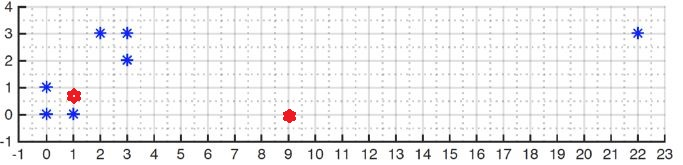
\includegraphics[scale=0.8]{images/4_2_1}
  \caption{Figures for k-means}\label{fig:kmeans}
\end{figure}

\begin{figure}[H]
  \centering
  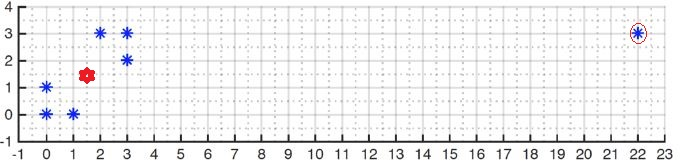
\includegraphics[scale=0.8]{images/4_2_2}
  \caption{Figures for k-means}\label{fig:kmeans}
\end{figure}


\end{enumerate}



  
